\section{Methodology}
\subsection{Probability distributions}
As explained before, the main goal of this project is simulating the SIR and SIS epidemic models into networks. Random numbers and, so, probability distributions are the basis of the project. We use 3 different distributions among all the paper: Poisson, power law and uniform. Except the second one, all the distributions used in this work are the ones implemented in the well-known \textit{random} standard library of C++. If the distribution is not specified somewhere in the paper, random numbers follow a uniform distribution then.

For the power law, we created ourselves the number generator that follows the distribution. Given a real random number $y$ between 0 and 1, the number generator returns the following: $$[(x_1^{1-\lambda}-(x_1^{1-\lambda}-x_0^{1-\lambda}))\cdot y]^\frac{1}{1-\lambda}$$
Where $x_0$ and $x_1$ are the maximum and minimum possible numbers, respectively, and $\lambda$ the exponent.

We tested the generator generating 10000 numbers with it and checking whether them follow a power law or not. You can see the results in figure~\ref{fig:powerlaw}. 

\begin{figure*}[hbtp]
    \centering
    \begin{subfigure}[b]{0.45\textwidth}
        \centering
          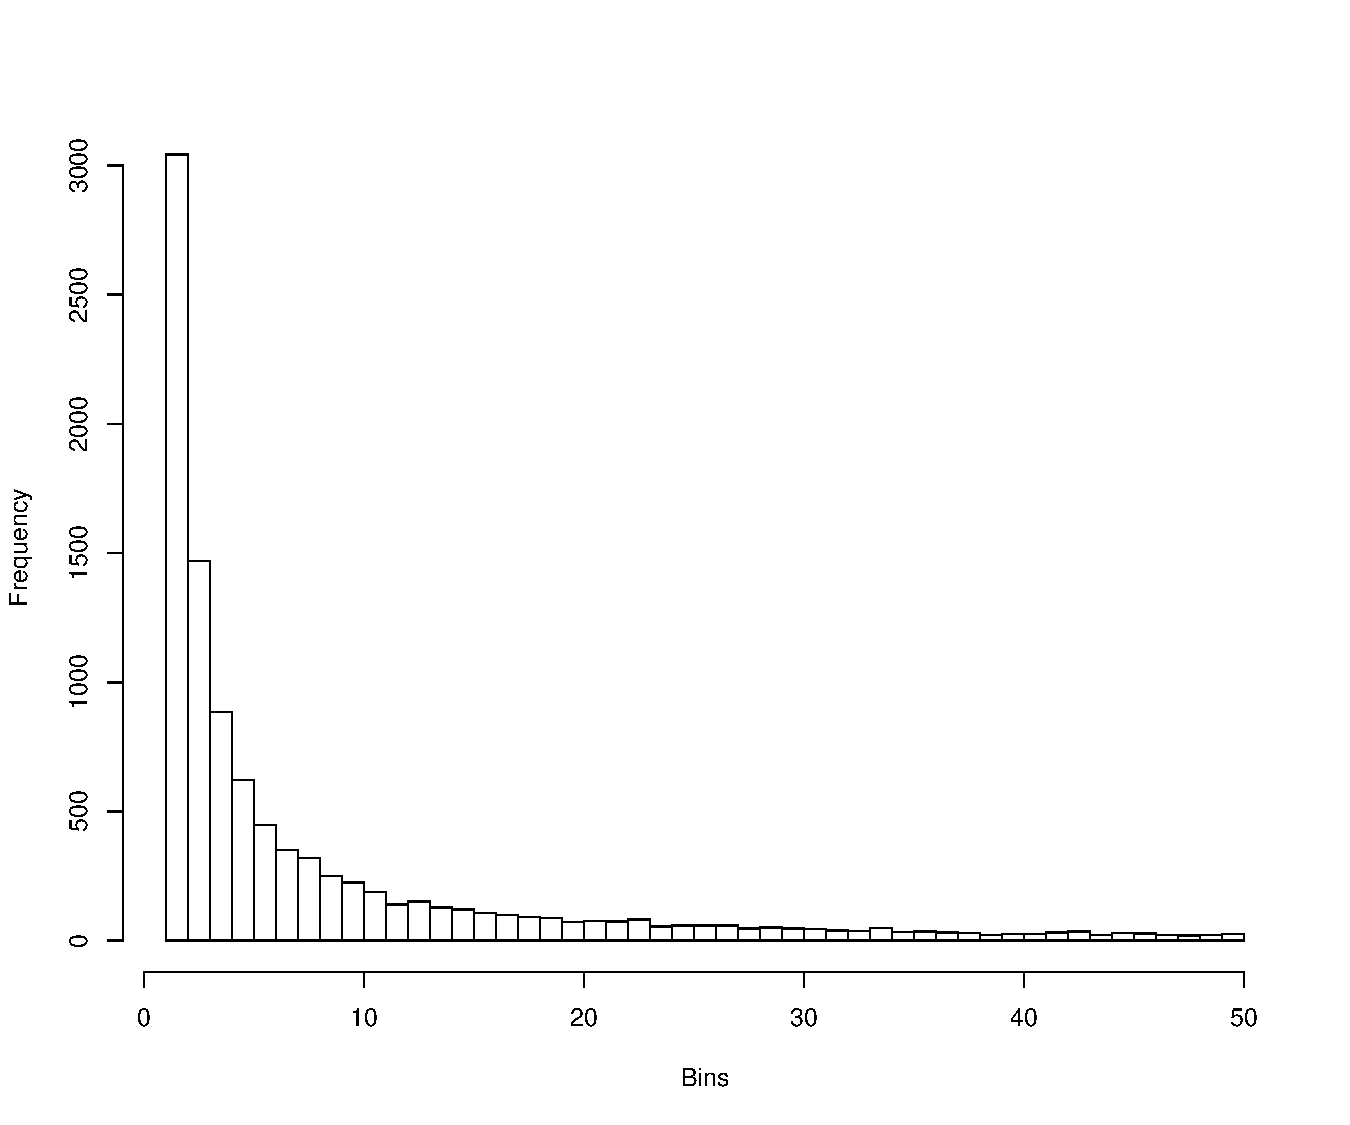
\includegraphics[width=\textwidth]{../img/power_law.pdf}
          \caption{Normal scale}
    \end{subfigure}
    \hspace{0.08\textwidth}
    \begin{subfigure}[b]{0.45\textwidth}
        \centering
          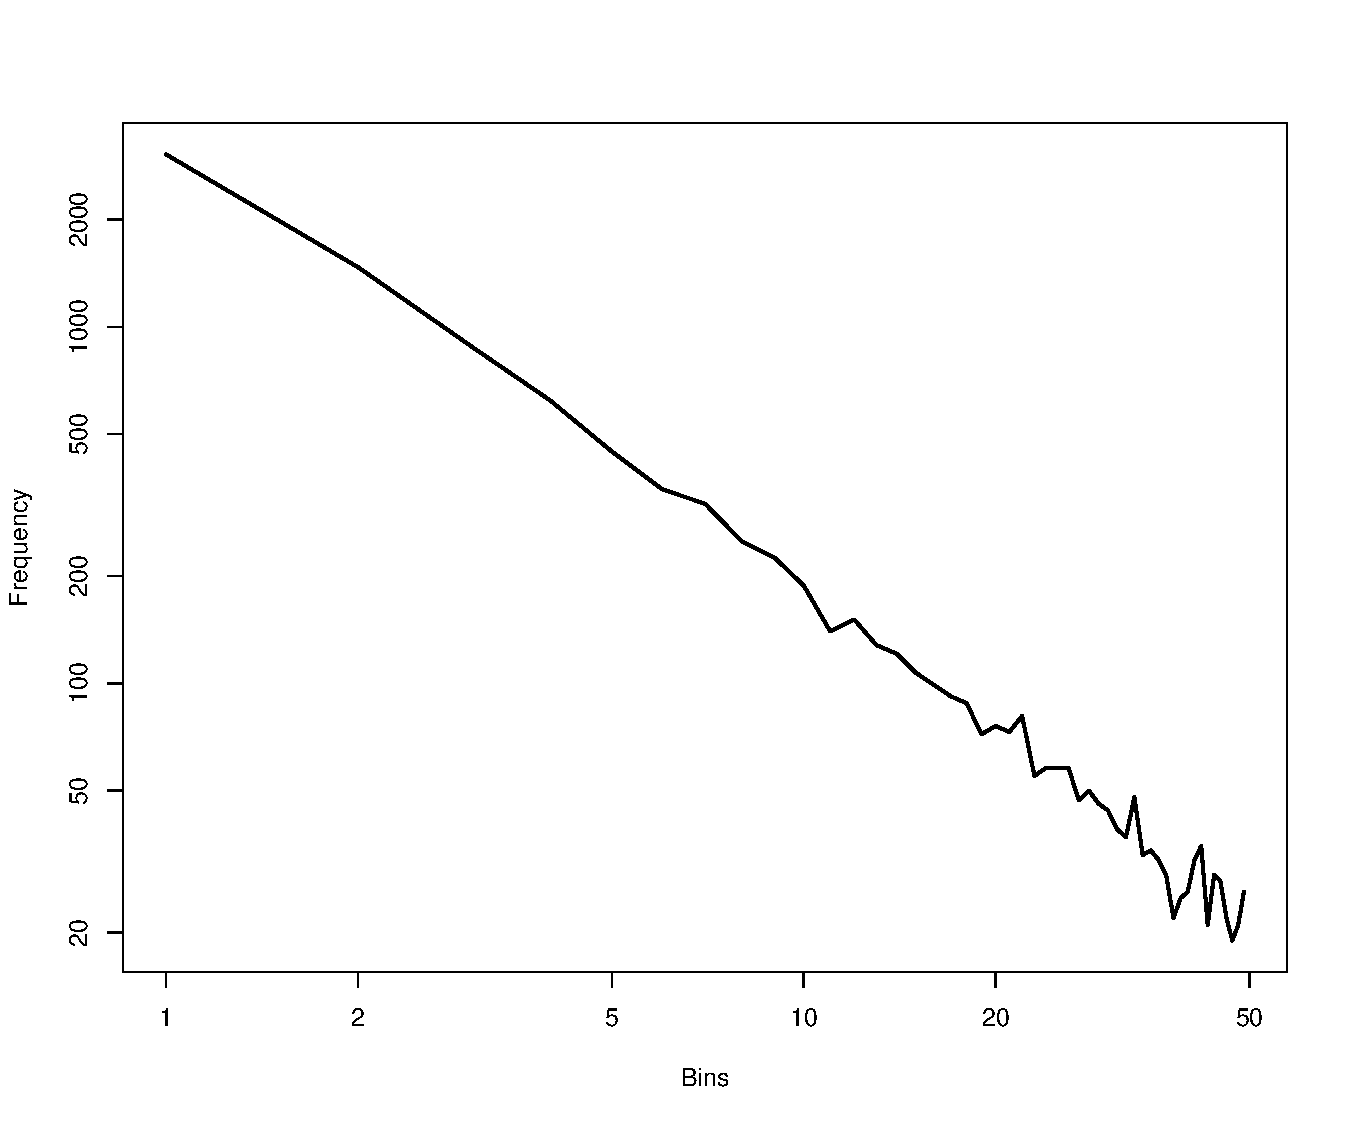
\includegraphics[width=\textwidth]{../img/power_law_log.pdf}
          \caption{Log scale (line histogram)}
    \end{subfigure}
    \caption{Generated numbers with our power law number generator. We divided all the possible values into 50 bins.}
    \label{fig:powerlaw}
\end{figure*}


\subsection{Network Generation}
Networks are obtained by first generating 10000 nodes with $k_i$ stubs ($0 \leq i < n$). Each $k_i$ is selected randomly using a Poisson or a power law distribution. The $l_i$ interaction events a node has are then distributed among its $k_i$ stubs. Again, each $l_i$ is randomly picked using a Poisson or power law distributions, or they are just $\delta \cdot k_i$. We refer to this as the delta distribution, though it is just a multiplication of $k_i$. Moreover, the interactions of a node are distributed among the stubs in the following way:
\begin{enumerate}
    \item Generate one real number $r_j$ between 0 and 1 for each stub ($0 \leq j < k_i$).
    \item Calculate the total sum. $$total = \sum_{j=0}^{k_i}r_j$$
    \item Each stub is then equal to $$\lfloor \frac{(l_i-k_i)\cdot r_j}{total}\rfloor$$
    With this, all (or almost all) the interactions are distributed.
    \item Distribute randomly the remaining interactions, if any.
\end{enumerate}
This process assigns a weight to each stub of a node according to its $l_i$.

After this, the adjacency matrix of the network is generated following this process:
\begin{enumerate}
    \item \textbf{Match}. Stubs are randomly matched together. To do this, we put all the stubs in a vector and we shuffle it. Then, each stub in a even position within the resultant vector is matched to the stub at its right, if there is one. If the stubs in a match are from the same node, we randomly select another stub of the vector and we try to swap it with one of the others. We repeat this process until all matched stubs are from different nodes.
    \item \textbf{Reject}. A match can be rejected if the weights of the stubs differ by more than one interaction event. In addition, matches are rejected if they differ by more than 10\% of the smaller weight involved to avoid biases in nodes with few links. If stubs with non-identical weighs are matched, i.e. they differ by 1, we assign randomly one of them to the weight of the connection.
    \item \textbf{Connect} For all accepted match, we sum its weight to the corresponding position of the adjacency matrix. We sum instead of assign the weight to the matrix in order to avoid checking that there not exist any match between the same nodes.
\end{enumerate}
Since this way of matching the nodes can lead to a lot of rejections, this process is repeated until it does not match any stub more in two consecutive iterations. Finally, we generate the adjacency list from the matrix to reduce the memory size, and because we can iterate through it faster.

\subsection{Infection Simulation}
To simulate the epidemic infection spread through the generated networks, we tested two different models: SIR and SIS.
\subsubsection{SIR}
The initials for this models stands for: Susceptible, Infected and Recovered. This simulate a disease that infects with probability $\mu_{SI}$, where this probability is dependent from how many contacts with infected hosts it is having. Basically, every node in susceptible state, can be infected by each connection with an infected host by a probability $\beta$. Then an infected host can recover with probability $\mu_{IR}$, where this probability is constant for all the nodes, in our case we set $\mu_{IR}=\gamma$. Finally when the host has ben recovered, it can't get infected again. So basically each host follows the state machine shown in figure \ref{fig:sir}.
\begin{figure}[htbp]
    \centering
    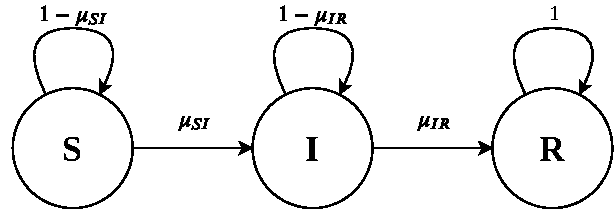
\includegraphics[width=\linewidth]{../img/SIR_model.pdf}
    \caption{SIR model representation.}
    \label{fig:sir}
\end{figure}

Assuming we have an adjacency list $W$, where each position is equal to the weight between the two nodes. In order to simulate this in an optimal way, at each time step, we go through all nodes of the network and do the following:
\begin{itemize}
    \item \textbf{If node i is Susceptible:} 
    \begin{itemize}
        \item[] $n=\sum_{j\in I}W_i,j$
        \item[] $\mu_{SI}=1-(1-\beta)^n$
        \item[] if $\mu_{SI}>real\_random(0,1)$: i is Infected
        \item[] else: i stays Susceptible  
    \end{itemize}
    \item \textbf{If node i is Infected:} 
    \begin{itemize}
        \item[] if $\gamma>real\_random(0,1)$: i is Recovered
        \item[] else: i stays Infected
    \end{itemize}
    \item \textbf{If node i is Recovered:} 
    \begin{itemize}
        \item[] i stays Recovered
    \end{itemize}
\end{itemize}
Note that $j\in I$ means that j is an infected node and the function $real\_random(0,1)$ gives a random value with an uniform distribution between 0 and 1.
\subsubsection{SIS}
The initials of this model stands for: Susceptible, Infected, Susceptible. This means that there is no Recovered state where the node is immune. Essentially the model to move from state S to I is exactly the same as in the SIR model, but this time when an infected node recovers, it simply become again a Susceptible node (see figure \ref{fig:sis}).
\begin{figure}[htbp]
    \centering
    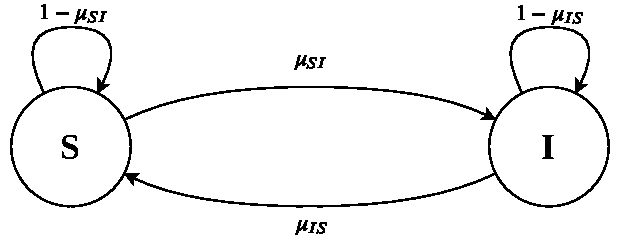
\includegraphics[width=\linewidth]{../img/SIS_model.pdf}
    \caption{SIS model representation.}
    \label{fig:sis}
\end{figure}

To simulate this we do like in SIR but, at each time step, we go through all nodes of the network and do the following:
\begin{itemize}
    \item \textbf{If node i is Susceptible:} 
    \begin{itemize}
        \item[] $n=\sum_{j\in I}W_i,j$
        \item[] $\mu_{SI}=1-(1-\beta)^n$
        \item[] if $\mu_{SI}>real\_random(0,1)$: i is Infected
        \item[] else: i stays Susceptible  
    \end{itemize}
    \item \textbf{If node i is Infected:} 
    \begin{itemize}
        \item[] if $\gamma>real\_random(0,1)$: i is Recovered
        \item[] else: i stays Infected
    \end{itemize}
\end{itemize}
\subsection{Experiments}
\label{ssec:experiments}
In our experiments, we test 6 different networks:
\begin{itemize}
    \item $P_k$ Poisson - $P_l$ Poisson
    \item $P_k$ power law - $P_l$ Poisson
    \item $P_k$ Poisson - $P_l$ power law 
    \item $P_k$ power law - $P_l$ power law
    \item $P_k$ Poisson - $P_l$ delta
    \item $P_k$ power law - $P_l$ delta
\end{itemize}
The parameters are:
\begin{itemize}
    \item $P_k$ Poisson: $<k> = 4$
    \item $P_l$ Poisson: $<l> = 8$
    \item $P_k$ power law: $\lambda_k=1.4$, $x_0=1$ and $x_1=22$
    \item $P_l$ power law: $\lambda_l=0.89$, $x_0=k$ and $x_1=22$
    \item $P_l$ delta: $\delta = 2$
\end{itemize}
We generated 20 networks for each of the mentioned configurations and in them we simulated 100 times each simulation model (SIR and SIS). We used the same parameters in both models, $\beta = 0.01$ and $\gamma = 0.004$.